\chapter{Planowanie, testowanie i wdrożenie}

Ostatni etap prac nad systemem FasterPost obejmował weryfikację spełnienia wymagań funkcjonalnych, analizę jakości kodu oraz przygotowanie procedur wdrożeniowych. W niniejszym rozdziale przedstawiono harmonogram realizacji projektu, macierz śledzenia wymagań (RTM) oraz szczegółową instrukcję uruchomienia środowiska produkcyjnego opartego na konteneryzacji.

\section{Harmonogram realizacji projektu}

Prace nad systemem zostały podzielone na etapy zgodnie z metodyką przyrostową. Kluczowe fazy obejmowały analizę wymagań, projektowanie architektury, implementację poszczególnych modułów (Backend/Frontend) oraz testy integracyjne. Rzeczywisty przebieg prac w czasie zobrazowano na wykresie Gantta (Rys. \ref{fig:gantt}).

\begin{figure}[htbp]
    \centering
    % Zakładam, że plik graficzny istnieje w tej ścieżce
    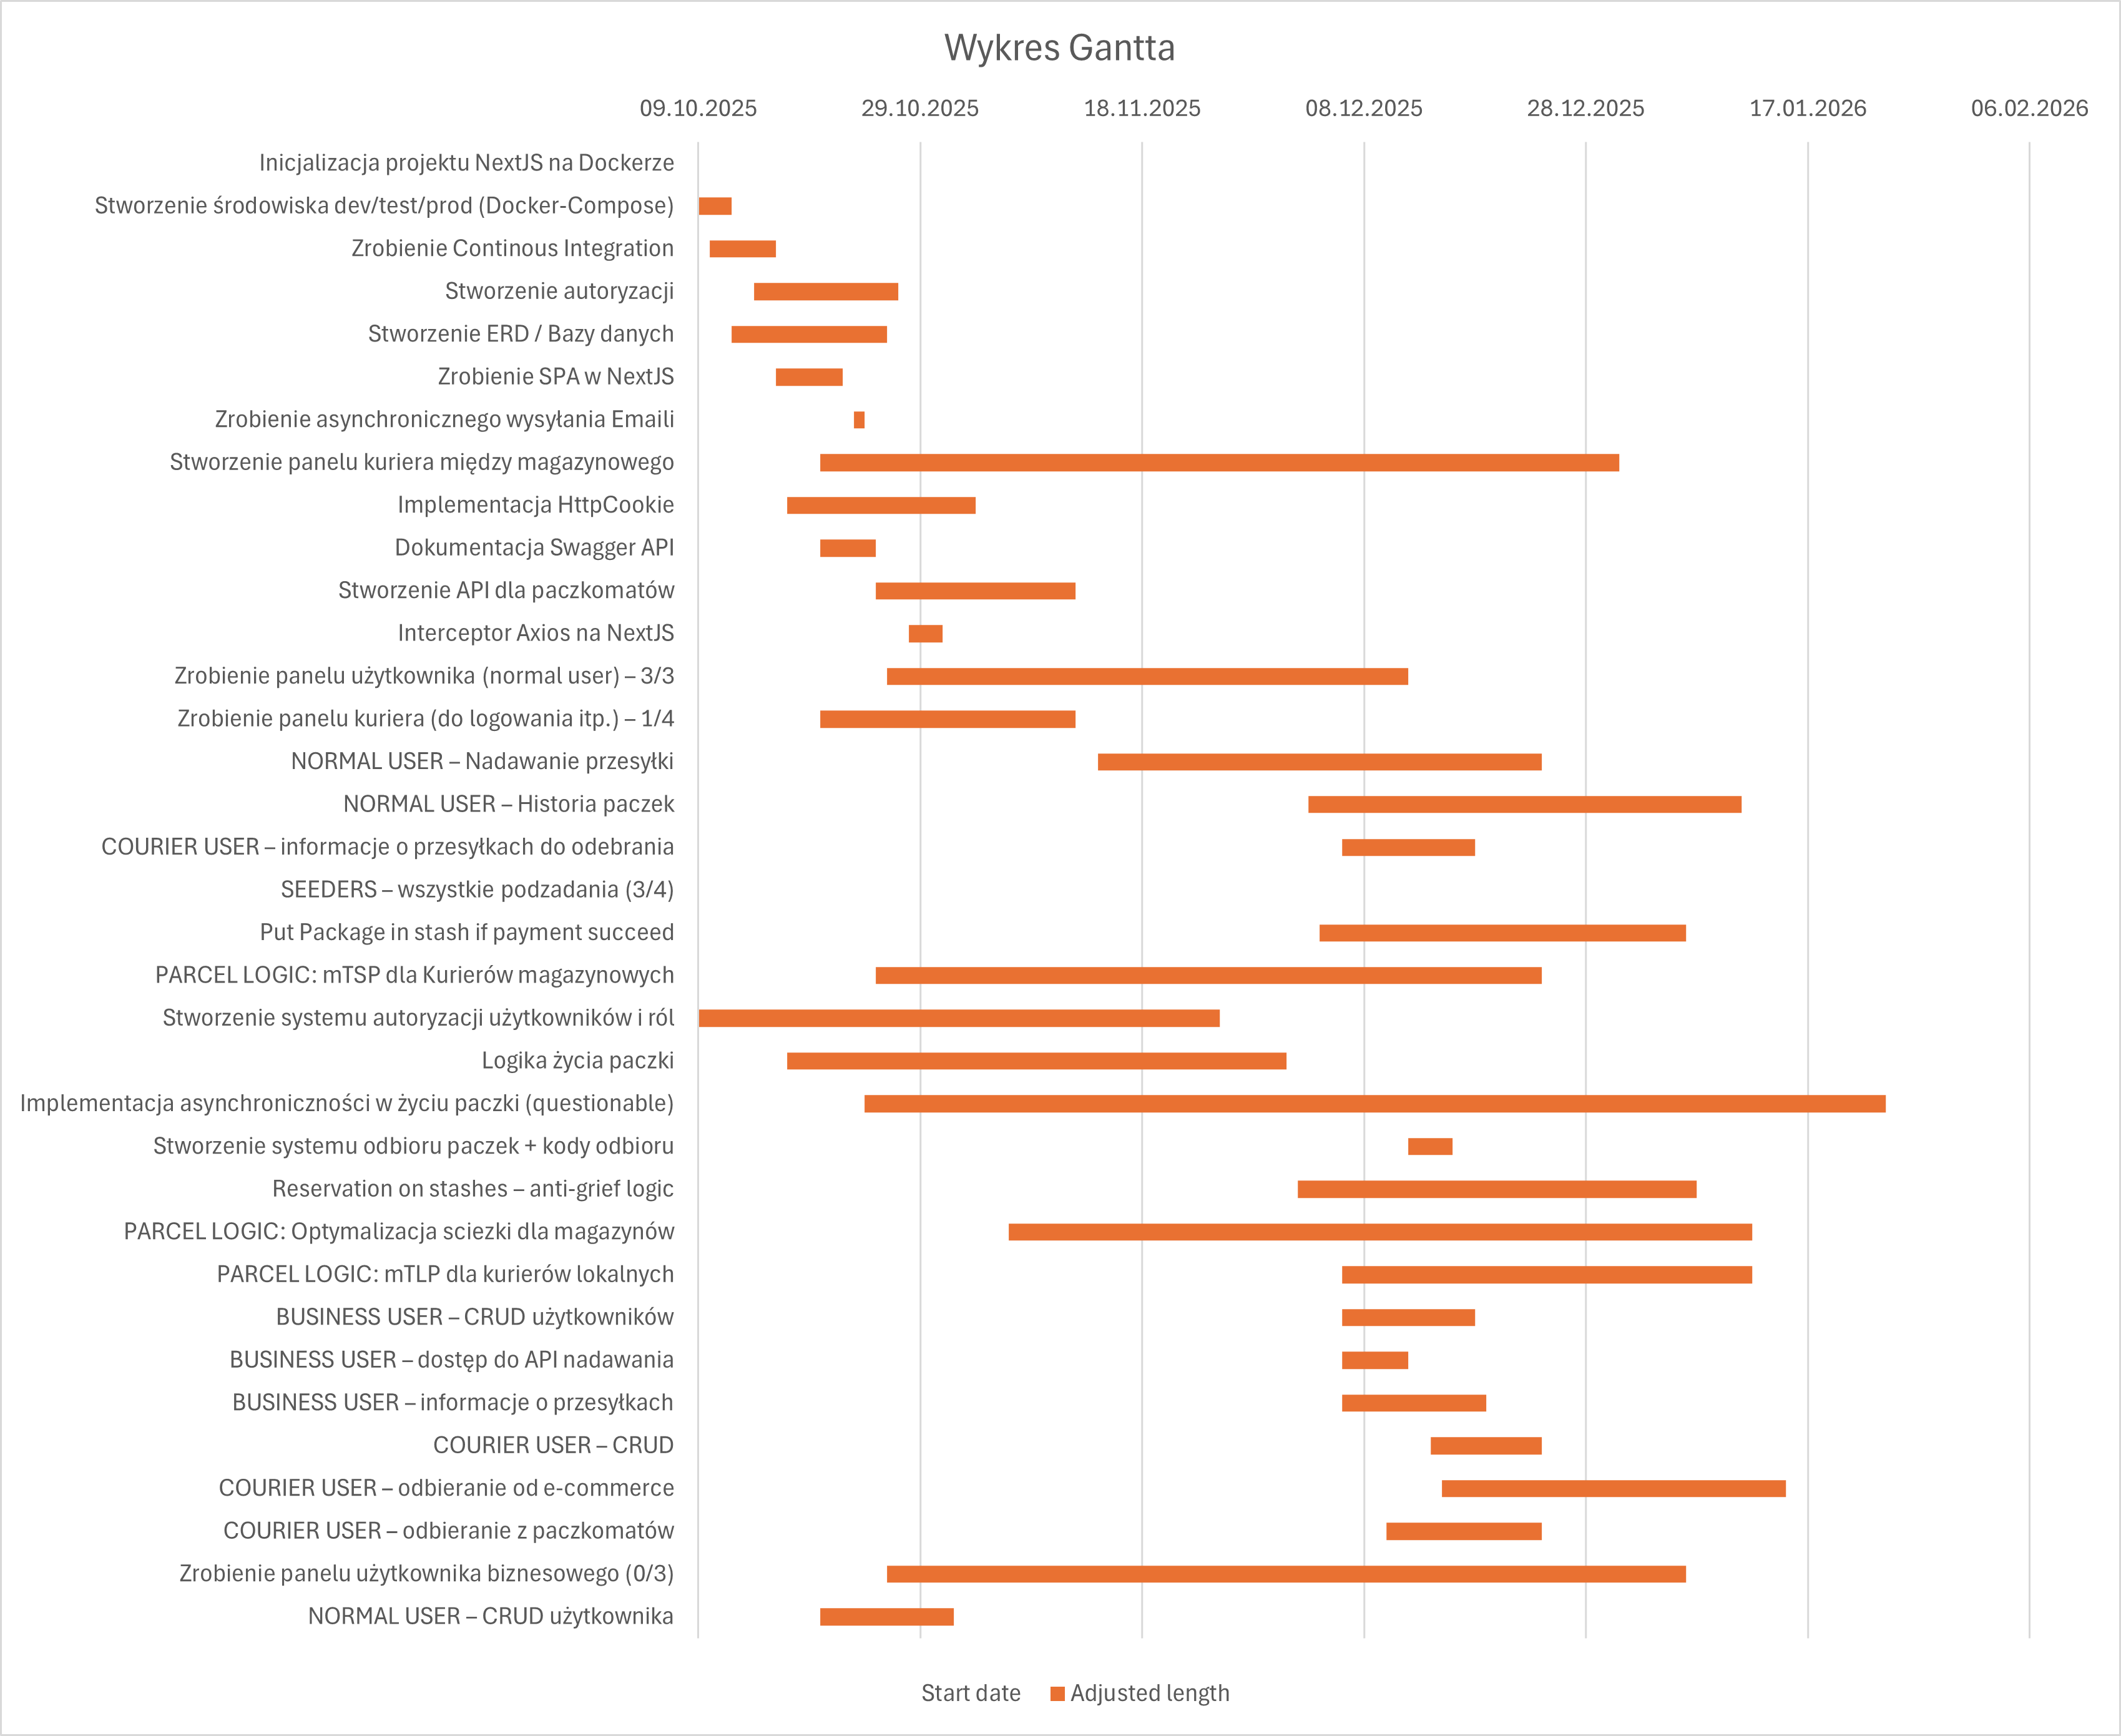
\includegraphics[width=1.0\textwidth]{../screenshots/gantt.png}
    \caption{Harmonogram realizacji projektu FasterPost (Wykres Gantta)}
    \label{fig:gantt}
\end{figure}

\section{Zapewnienie jakości i testy}

W celu zagwarantowania niezawodności systemu, zastosowano strategię testowania obejmującą testy jednostkowe (Unit Tests) oraz integracyjne (Integration Tests). Proces ten został zautomatyzowany przy użyciu potoku CI/CD (GitHub Actions), zdefiniowanego w pliku \texttt{.github/workflows/tests.yml}. Każda zmiana w kodzie (Push/Pull Request) inicjuje automatyczne uruchomienie zestawu testów w izolowanym środowisku kontenerowym.

\subsection{Macierz Śledzenia Wymagań (RTM)}

Poniższa tabela (Tab. \ref{tab:rtm}) przedstawia powiązanie zdefiniowanych wymagań funkcjonalnych z konkretnymi przypadkami testowymi zaimplementowanymi w katalogu \texttt{backend/tests/}. Pozwala to na weryfikację pokrycia wymagań testami.

\begin{table}[htbp]
    \centering
    \caption{Macierz Śledzenia Wymagań (Requirements Traceability Matrix)}
    \label{tab:rtm}
    \small % Zmniejszenie fontu, aby tabela była bardziej zwarta
    \renewcommand{\arraystretch}{1.3} % Lekkie zwiększenie odstępów w wierszach dla czytelności
    \begin{tabularx}{\textwidth}{|c|p{3.5cm}|p{3.5cm}|X|}
        \hline
        \textbf{ID} & \textbf{Wymaganie Funkcjonalne} & \textbf{Klasa / Plik Testowy} & \textbf{Cel testu i weryfikacja} \\ \hline
        FR-01 & Rejestracja użytkownika i walidacja haseł & \texttt{RegistrationTestCase} & Sprawdzenie unikalności e-mail oraz walidacja długości i siły hasła. \\ \hline
        FR-02 & Weryfikacja konta przez e-mail & \texttt{EmailVerificationTestCase} & Weryfikacja działania tokenów aktywacyjnych oraz ich wygasania. \\ \hline
        FR-03 & Logowanie i zarządzenie sesją & \texttt{LoginTestCase} & Sprawdzenie poprawności generowania i rotacji tokenów dostępu. \\ \hline
        FR-04 & Wylogowanie użytkownika & \texttt{LogoutTestCase} & Weryfikacja unieważnienia tokena sesji po stronie serwera. \\ \hline
        FR-05 & Odzyskiwanie dostępu do konta & \texttt{PasswordResetTestCase} & Test pełnego procesu zmiany zapomnianego hasła przez e-mail. \\ \hline
        FR-06 & Bezpieczeństwo sesji (Expiring Token) & \texttt{ExpiringTokenTestCase} & Weryfikacja automatycznej deautoryzacji po wygaśnięciu tokena. \\ \hline
        FR-07 & Konfiguracja 2FA (TOTP) & \texttt{TOTPViewTestCase} & Sprawdzenie generowania sekretów TOTP i weryfikacji kodów. \\ \hline
        FR-08 & Logowanie z drugim składnikiem (MFA) & \texttt{LoginTOTPTestCase} & Wymuszenie podania kodu TOTP podczas procesu logowania (status 206). \\ \hline
        FR-09 & Logistyka: Priorytetyzacja FIFO & \texttt{LocalRoutingServiceTests} & Alokacja paczek w szafkach z uwzględnieniem czasu przybycia do magazynu. \\ \hline
        FR-10 & Logistyka: Obsługa punktów PUDO & \texttt{LocalRoutingServiceTests} & Realizacja dostaw do punktów bez wymogu posiadania wolnej skrytki. \\ \hline
    \end{tabularx}
\end{table}

\subsection{Analiza wyników testów}

Testy wydajnościowe algorytmów logistycznych wykazały, że dla standardowego zestawu danych (50 paczek na pojazd, miasto średniej wielkości):
\begin{itemize}
    \item Algorytm CVRP (Nearest Neighbor) generuje trasę w czasie poniżej 200ms.
    \item Algorytm K-Means (podział na strefy) dla 100 paczkomatów wykonuje się w czasie poniżej 2 sekund (proces jednorazowy/rzadki).
    \item Weryfikacja dostępności skrytek (zapytania do bazy danych) jest optymalizowana przez indeksy na kolumnach \texttt{is\_empty} i \texttt{reserved\_until}.
\end{itemize}

\section{Instrukcja wdrożenia i uruchomienia}

System FasterPost został zaprojektowany z myślą o łatwym wdrażaniu przy użyciu technologii Docker. Poniżej przedstawiono procedurę uruchomienia środowiska deweloperskiego oraz produkcyjnego.

\subsection{Wymagania wstępne}

Do poprawnego działania systemu wymagane jest zainstalowanie następującego oprogramowania:
\begin{itemize}
    \item Docker Engine (wersja 20.10+)
    \item Docker Compose (wersja 1.29+)
\end{itemize}

\subsection{Konfiguracja zmiennych środowiskowych}

Przed uruchomieniem kontenerów należy skonfigurować plik \texttt{.env} w katalogu głównym projektu (lub w katalogu \texttt{backend/}). Przykładowa konfiguracja:

\begin{lstlisting}[language=bash, caption=Przykładowa konfiguracja pliku .env]
DEBUG=1
SECRET_KEY=django-insecure-change-me-in-prod
ALLOWED_HOSTS=localhost,127.0.0.1

# Baza Danych
DB_NAME=fasterpost
DB_USER=postgres
DB_PASSWORD=postgres
DB_HOST=db
DB_PORT=5432

# Redis & Celery
REDIS_URL=redis://redis:6379/0

# Integracje zewnetrzne
STRIPE_PUBLIC_KEY=pk_test_...
STRIPE_SECRET_KEY=sk_test_...
\end{lstlisting}

\subsection{Uruchomienie kontenerów}

Proces budowania obrazów i uruchamiania usług odbywa się za pomocą jednej komendy. Docker Compose automatycznie pobierze obrazy bazowe (Python, Node.js, Postgres, Redis) i zbuduje aplikację.

\begin{lstlisting}[language=bash, caption=Komenda uruchamiająca środowisko]
docker-compose up --build
\end{lstlisting}

Po zakończeniu procesu budowania, usługi będą dostępne pod następującymi adresami:
\begin{itemize}
    \item \textbf{Frontend (Klient):} http://localhost:80
    \item \textbf{Backend (API):} http://localhost:8000
    \item \textbf{Dokumentacja API (Swagger):} http://localhost:8000/api/schema/swagger-ui/
\end{itemize}

\subsection{Inicjalizacja danych (Seeding)}

Aby system był w pełni funkcjonalny (posiadał zdefiniowane magazyny, paczkomaty, strefy i użytkowników testowych), konieczne jest przeprowadzenie procesu "seedowania" bazy danych. Należy wykonać poniższe komendy wewnątrz kontenera backendu:

\begin{lstlisting}[language=bash, caption=Skrypty inicjalizujące dane testowe]
# 1. Migracje schematu bazy danych
docker-compose run web python manage.py migrate

# 2. Tworzenie magazynow centralnych (Hubow)
docker-compose run web python manage.py seed_warehouses

# 3. Tworzenie polaczen miedzy magazynami (Graf logistyczny)
docker-compose run web python manage.py seed_logistics

# 4. Tworzenie uzytkownikow (Admin, Kurierzy, Klienci)
docker-compose run web python manage.py seed_accounts

# 5. Generowanie stref (Algorytm K-Means)
docker-compose run web python manage.py seed_zones

# 6. Generowanie paczkomatow i skrytek
docker-compose run web python manage.py seed_local_delivery
\end{lstlisting}

Po wykonaniu tych kroków system jest gotowy do pracy, a użytkownik może zalogować się na konto administratora lub klienta testowego.

\section{Podsumowanie wdrożenia}

Proces wdrożenia oparty na konteneryzacji zapewnia spójność środowiska uruchomieniowego niezależnie od systemu operacyjnego hosta. Wykorzystanie Docker Compose ułatwia orkiestrację wielu usług (Baza danych, Redis, Celery Worker, Backend, Frontend), co znacząco skraca czas potrzebny na konfigurację nowej instancji systemu FasterPost.